\section{Введение}%\addcontentsline{toc}{section}{Введение}
Нуклеосинтезом называют совокупность протекающих в естественных условиях ядерных процессов, приводящих к образованию атомных ядер. Исследование механизмов нуклеосинтеза является актуальной задачей современной физики, так как они определяют распространенность ядер химических элементов во Вселенной и играют важную роль в астрофизике. Нуклеосинтез сопровождает эволюцию Вселенной с самого ее рождения. В первичном, дозвездном нуклеосинтезе, начавшемся уже в первые секунды после Большого взрыва, стали возникать легчайшие ядра, изотопы водорода и гелия. Наблюдаемое сегодня подавляющее преобладание ядер ${}^1$H и ${}^4$He сложилось именно за счет дозвездного нуклеосинтеза. В звездном нуклеосинтезе, начавшемся приблизительно через 1 млрд лет с появлением первых звезд, в результате стадий термоядерного горения, чередующихся со стадиями гравитационного сжатия, образуются химические элементы вплоть до железа. 

Процессы, приводящие к образованию более тяжелых элементов, представляют большой интерес для современной физики. Как известно, нуклеосинтез ядер тяжелее железа энергетически невыгоден из-за так называемого <<железного пика>> --- максимума зависимости удельной энергии связи от массового числа. Термоядерное горение не может быть источником таких изотопов, за их появление отвечают другие механизмы. По-видимому, важнейшим из них является процесс быстрого захвата нейтронов.

\begin{figure}[!b]
  \centering
  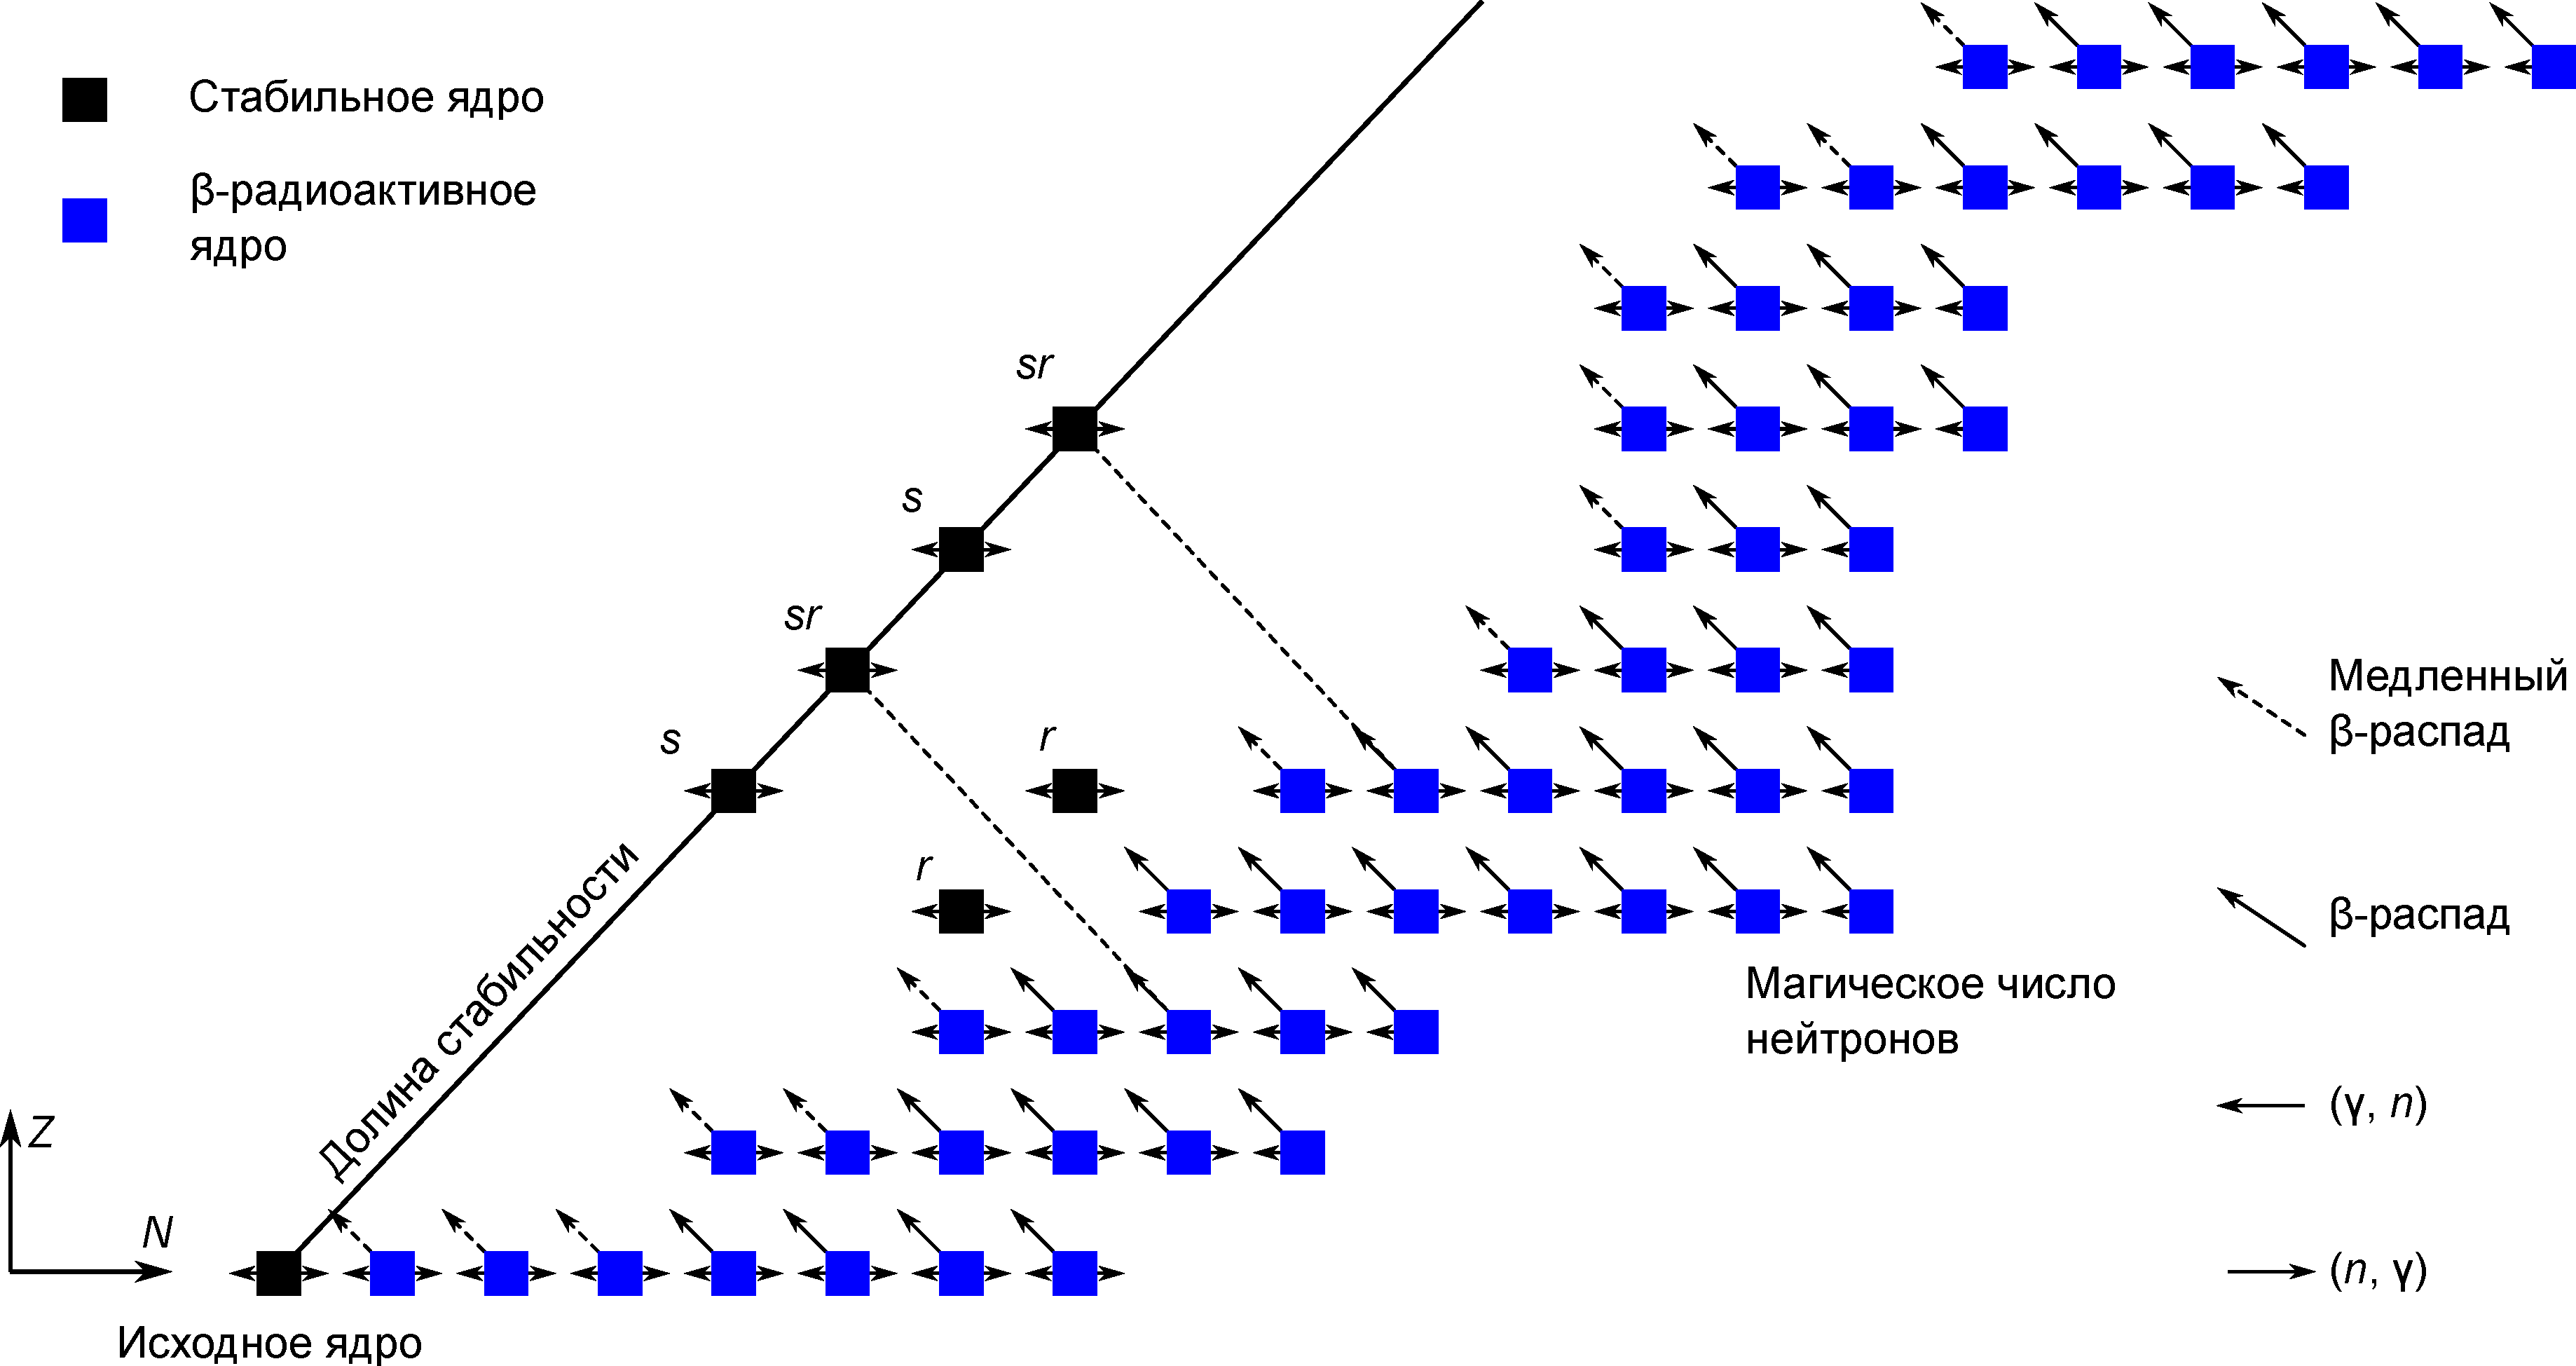
\includegraphics[width=0.8\textwidth]{../pics/tracks.pdf}
  \caption{Схематическое изображение ядерных реакций астрофизического $r$-процесса.}
  \label{fig:tracks}
\end{figure}

\begin{figure}[!b]
  \centering
  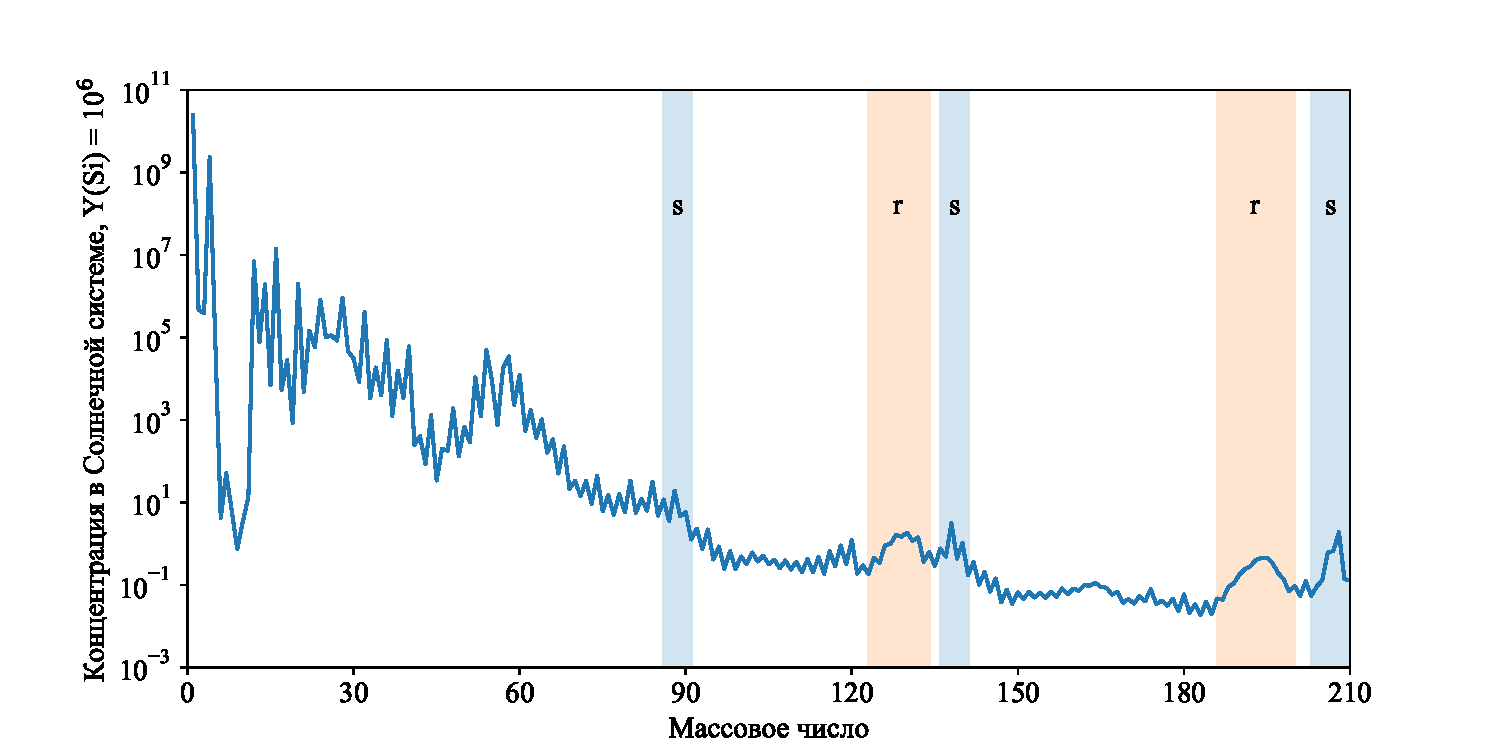
\includegraphics[width=0.8\textwidth]{../pics/lodders.pdf}
  \caption{Массовое распределение ядер в Солнечной системе по данным~\cite{lodders2003}, масса изотопов Si принята равной $10^6$. Оранжевым отмечены пики $r$-процесса, синим --- пики $s$-процесса (согласно~\cite{cowan2021}).}
  \label{fig:lodders_vs_ame}
\end{figure}

\subsection{Нуклеосинтез тяжелых элементов}
Астрофизическим $r$-процессом, или процессом быстрого нейтронного захвата, называется механизм нуклеосинтеза, в ходе которого исходное ядро поглощает большое число нейтронов и, оказавшись в области нейтронного избытка, испытывает слабые распады. Схематично превращения, происходящие с ядром в $r$-процессе, показаны на рис.~\ref{fig:tracks}. В результате масса ядра увеличивается за счет поглощенных нейтронов, а $\beta^-$-распады приводят к образованию химического элемента с большим зарядовым числом. В $r$-процессе скорости нейтронного захвата на порядки превышают скорости $\beta^-$-распадов, что обеспечивает стремительный набор массы и значительное смещение в область нейтронного избытка. Для достижения необходимой интенсивности поглощения нейтронов требуется высокая плотность их потока, около 150 нейтронов на одно зародышевое ядро, и температуры вещества свыше 1~ГК. Подобные условия являются экстремальными даже по меркам астрофизики. Они могут реализовываться лишь в таких катастрофических явлениях, как взрывы сверхновых, слияния двух нейтронных звезд или нейтронной звезды и черной дыры.

По современным представлениям, именно $r$-процесс обеспечивает возникновение основной массы ядер химических элементов тяжелее железа во Вселенной. Процесс медленного нейтронного захвата, или $s$-процесс, отличающийся от $r$-процесса значительно меньшей интенсивностью поглощения нейтронов и, соответственно, характерными временами порядка сотен лет, требует не столь исключительных астрофизических условий и обеспечивает образование ядер вблизи долины стабильности вплоть до свинца и висмута. Тем не менее $s$-процессом нельзя объяснить существование более тяжелых ядер, а также нейтроноизбыточных изотопов, слишком удаленных от долины стабильности. Некоторое количество обойденных протоноизбыточных изотопов возникает в $p$-процессе, механизме взрывного нуклеосинтеза, представляющем собой последовательности фотоядерных реакций и поглощений заряженных частиц. Однако выходы $p$-процесса малы по сравнению с $s$- и $r$-процессами. Кроме того, для синтеза $p$-изотопов требуется наличие достаточно тяжелых стабильных ядер, достаточное число которых может образоваться только в результате процессов нейтронного захвата. 

На рис.~\ref{fig:lodders_vs_ame} представлено массовое распределение ядер химических элементов в Солнечной системе, построенное по данным~\cite{lodders2003}. Виден избыток легчайших изотопов с $A \leq 4$, родившихся в первичном нуклеосинтезе, за которым следует минимум, соответствующий изотопам Li, Be и B. С массового числа 12 начинается область ядер, рождающихся в основном за счет термоядерного горения звездного вещества, в частности, pp- и CNO-циклов. Видно, что начиная с массовых чисел $54 - 58$, соответствующих <<железному пику>>, начинается существенное снижение концентраций изотопов. В области более тяжелых ядер нуклеосинтез целиком обеспечивается $s$- и $r$-процессами. На рис.~\ref{fig:lodders_vs_ame} отмечены характерные пики, соответствующие магическим числам нейтронов 50, 82 и 126, что является указанием на высокий вклад процессов нейтронного захвата в нуклеисинтез. Более узкие пики образуются благодаря $s$-процессу, который протекает вблизи долины стабильности, в то время как $r$-процесс рождает сверх-нейтроноизбыточные ядра. Для таких экзотических изотопов могут преобладать уже не $\beta^-$-распады, протекающие без потери массы, а слабые распады с вылетом нейтронов, что приводит к размыванию и смещению пика $r$-процесса в область меньших масс.

На сегодняшний день слияние двух сверхкомпактных астрофизических объектов, двух нейтронных звезд (\nsm{}) или нейтронной звезды и черной дыры звездной массы, принято считать основным сценарием протекания $r$-процесса~\cite{theilemann2017}. Сопровождающий слияние выброс нагретого вещества является подходящей средой для образования наиболее тяжелых нерукотворных химических элементов за счет быстрого нейтронного захвата. В пользу выброса вещества \nsm{} как важного источника $r$-изотопов говорит избыток нейтронов (средняя доля протонов в выбросе составляет $Y_e \equiv \expval{Z/A} \approx 0.1$~\cite{kajino2019}), а также сходство распространенностей тяжелых изотопов с $A > 120$ в симуляциях этого сценария нуклеосинтеза с распространенностями в Солнечной системе (например,~\cite{freiberghaus1999,goriely2011}). При этом нельзя сказать, что сценарий \nsm{} полностью объясняет распределение $r$-изотопов во Вселенной. В ряде работ (например,~\cite{honda2006,qian2007,hansen2014}) отмечаются особенности состава старых звезд малой металличности, указывающие на заметный вклад слабого $r$-процесса, который может протекать, например, при вспышках сверхновых.  

В обзорах~\cite{arnould2007,kajino2019,cowan2021} подробно обсуждается механизм астрофизического $r$-процесса и текущий прогресс его изучения.

\subsection{Особенности изучения $r$-процесса}
Экстремальные условия протекания $r$-процесса делают его экспериментальное исследование практически невозможным. Основным источником эмпирических сведений об этом механизме на сегодняшний день являются распространенности ядер химических элементов в Солнечной системе (см. рис.~\ref{fig:lodders_vs_ame}), известные благодаря исследованиям состава метеоритов-хондритов, сформировавшихся из вещества дозвездного газопылевого облака. Также важным источником сведений об $r$-процессе является исследование спектрального состава звезд.

Из-за невозможности воспроизведения условий астрофизического синтеза тяжелых ядер в лаборатории основным методом изучения $r$-процесса становится компьютерное моделирование. С его помощью стремятся объяснить наблюдаемые распространенности ядер в Солнечной системе. При этом само моделирование $r$-процесса, сводящееся к решению системы дифференциальных уравнений, сопряжено с рядом трудностей: огромными размерами системы, разбросом значений скоростей реакций, неопределенностью входных параметров.

Входными параметрами симуляции $r$-процесса являются термодинамические характеристики среды и свойства задействованных в нуклеосинтезе ядер и ядерных реакций. Макроскопические параметры, такие как плотность и температура звездного вещества, в основном известны из астрофизических моделей. Результаты таких расчетов слияния нейтронных звезд представлены в работах~\cite{rosswog1999,rosswog2013}. В работах~\cite{korobkin2012,rosswog2014,kullman2021} вместе с моделированием слияния нейтронных звезд проводятся симуляции синтеза ядер в $r$-процессе.

Большую трудность представляет получение точных значений ядерных параметров моделирования $r$-процесса. Как показано на рис.~\ref{fig:tracks}, путь $r$-процесса лежит значительно ниже долины стабильности. Этот механизм нуклеосинтеза задействует экзотические нейтроноизбыточные ядра, экспериментальное изучение которых в лабораторных условиях представляется невозможным. Характеристики $r$-изотопов и реакций их образования приходится получать при помощи теоретических моделей. При этом различные ядерные модели могут давать существенно разные результаты для экзотических изотопов, например, при расчете энергий связи~\cite{sobiczewski2018}. Неопределенности энергий связи $r$-изотопов могут существенно сказываться на результатах расчета $r$-процесса, на что указывается, например, в работах~\cite{goriely2001,brett2012}.

Целью настоящей работы является определение чувствительности модели $r$-процесса к неопределенностям расчета масс нейтроноизбыточных ядер. Для этого нами были рассмотрены результаты трех расчетов масс нейтроноизбыточных ядер, выполненных при помощи различных ядерных моделей. При помощи этих теоретических значений масс были проведены расчеты сечений реакций нейтронного захвата и построены библиотеки астрофизических ядерных реакций, в которых учтено изменение границ области существования ядер в зависимости от используемой массовой модели. Уделено также внимание $\beta^-$-распадам, играющим большую роль в $r$-процессе. Полученные библиотеки реакций использованы при симуляции $r$-процесса в реалистичном астрофизическом сценарии слияния двух нейтронных звезд. Различия результирующих массовых распределений $r$-изотопов позволили оценить влияние неопределенностей теоретических значений масс нейтроноизбыточных ядер на моделирование $r$-процесса.
